\documentclass[article,oneside,a4paper,12pt]{memoir}

\usepackage[margin=1in,bottom=1.5in,footskip=45pt]{geometry}
\usepackage{fontspec}
\usepackage[calc,english]{datetime2}

\usepackage{graphicx}
\usepackage[export]{adjustbox}
\graphicspath{ {./images/} }

\usepackage{float}
\usepackage{booktabs}
\usepackage{multicol}
\usepackage{multirow}
\usepackage{adjustbox}

\usepackage[backend=biber,style=authoryear,citestyle=authoryear-comp]{biblatex}
\addbibresource{references.bib}

\setlength{\parindent}{0pt}
\nonzeroparskip

\newcommand{\possessivecite}[1]{\citeauthor{#1}'s (\citeyear{#1})}

\counterwithout{section}{chapter}
\setsecnumdepth{subsection}

\setmainfont{Libertinus Serif}

\DTMnewdatestyle{eurodate}{%
    \renewcommand{\DTMdisplaydate}[4]{%
        \number##3.\nobreakspace%           day
        \DTMmonthname{##2}\nobreakspace%    month
        \number##1%                         year
    }%
    \renewcommand{\DTMDisplaydate}{\DTMdisplaydate}%
}

\DTMsetdatestyle{eurodate}

\title{Mining Sentiments \& Arguments for Climate Change Tweet Classification}
\author{Bethany E. Toma}
\date{\today}

\begin{document}

\maketitle

\section{Introduction}

Incorporation of discourse features into sentiment and argument mining has been more and more popular in the NLP space. Twitter data exhibits a particular challenge here, due to the short nature of its ``documents'' as well as its general messiness and the unique qualities of its lexicon, such as the use of hashtags and emoicons. Past work has, however, applied use of lightweight algorithmic discourse analysis to Twitter data to improve its performance on other tasks, such as sentiment analysis \parencite{coling2012}. Here, we choose to extend one such method by applying it rather to opinion classification as opposed to binary positive-negative sentiment classification, specifically on the stances of tweets about climate change. By comparing performance of this discourse analysis method, which has been shown to succeed in binary sentiment analysis tasks on similar Twitter data, with simple non-discourse-aware bag-of-words methods, we can assess how well the method adapts to a new task and a slightly different domain of data.

\section{Methodology}

This project consisted of roughly two parts: (1) a crowd study run to annotate the unannotated Twitter data for use in opinion mining and (2) the training and comparison of classifier models with and without discourse features on this annotated data. A third part of the project, in which this approach was compared to fine-tuning a large neural model like BERT, was planned but not completed. In this section, each of these portions of the project will be discussed in detail.

\subsection{Crowd Study}

For this study, we were provided with a dataset of several million tweets related to climate change by Prof. Dr. Stede. As a result, we chose to focus this project on training a classifier to distinguish between those tweets written by someone who believed in anthropogenic climate change and those written by climate change deniers. We first filtered the Twitter data to remove duplicates, retweets, and any tweets containing links to images, websites, or other tweets. While this removed a large portion of our data, we felt it was necessary to remove instances in which even a human would struggle to classify a given tweet with the amount of context given. Consider the hypothetical tweet depicted in Figure \ref{fig:hypothetical}---without knowing the contents or title of the linked article, it's impossible to tell whether the author of this tweet believe in or denies climate change.

\begin{figure}[htb]
    \centering
    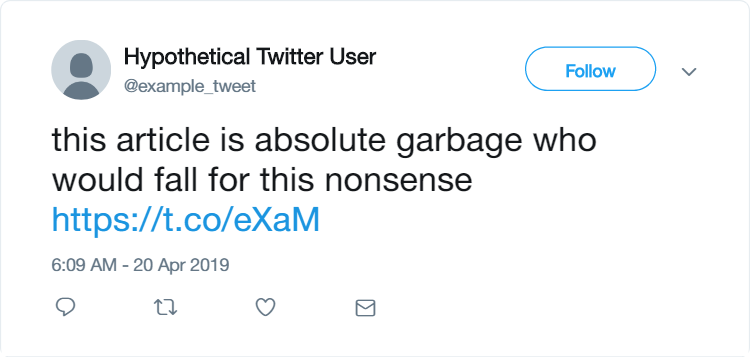
\includegraphics[width=0.8\textwidth, frame]{hypothetical-tweet}
    \caption{Hypothetical tweet with too little context for a human annotator (created using TweetGen Beta-0.2.0)}
    \label{fig:hypothetical}
\end{figure}

On Twitter itself, a user would be able to get a clearer picture of the author's opinion due to the inclusion of an embedded version of the link, which would feature the title and description of the linked webpage. While including this information for annotators would be possible using HTTP requests, doing so on such a large dataset would take an infeasibly large amount of time. While even tweets that do not contain links can be ambiguous in this regard without further context, we hoped to reduce the proportion of difficult-to-classify tweets in the data by removing tweets that contained links.

The resulting dataset consisted of just under one million tweets. These tweets had already had already been anonymized, including removal of \@-mentions, and tokenized (with tokens separated by spaces in the final product). However, none of these tweets had been annotated in any way, creating a pretty obvious problem for training a classifier. As a result, we began a crowd study in which human annotators would classify 1999 of these tweets by whether their author believed in climate change or not.

The survey through which annotation was performed was created and hosted using the SoSci Survey online tool, and 118 participants were solicited using the Prolific online platform. Each participant annotated 100 to 110 randomly-selected tweets, including five test tweets used to assess the quality of annotation. If an annotator did not get a score of at least 3/5 correct on the test tweets, their annotations were excluded. Based on this, 11 participants were excluded, with 107 participants remaining. For each tweet, participants selected ``yes,'' ``no,'' or ``unsure'' in response to the question ``Based solely on the text of this tweet, does the person who tweeted this believe in climate change?'' 

\begin{figure}[hbt]
    \begin{adjustbox}{width=1.2\textwidth,center=\textwidth}
    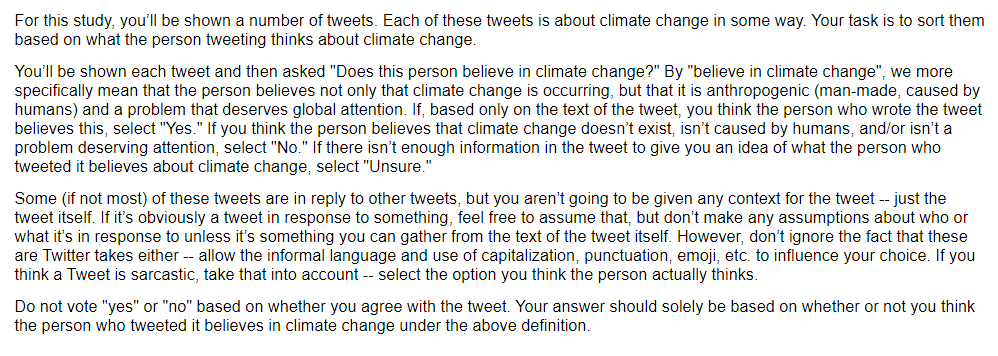
\includegraphics[width=1.2\textwidth,frame]{annotation-guidelines}
    \end{adjustbox}
        \caption{Guidelines given to human annotators for crowd study}
        \label{fig:annotation}
    \end{figure}

Annotators were presented with guidelines at the beginning of the study regarding what was meant when they were asked whether the author of a tweet ``believes in climate change.'' The exact form of these guidelines as shown to the participants is shown in Figure \ref{fig:annotation}. Participants were then asked whether they themselves believed in climate change according to the definition given. Of the participants whose annotations were not excluded due to poor responses on the test tweets, 100 answered ``yes'' while 7 answered ``no.'' Participants responses were not excluded solely on the basis of whether they believed in climate change or not.

Upon the conclusion of the study, each tweet was assigned a label based on the annotations given in the crowd study. If at least one label was assigned to the same tweet by at least three annotators and the most common label was assigned at least two times more than the non-``unsure'' labels, the tweet was assigned that label. If both ``unsure'' and one of the other labels tied for most common label and the difference between the two non-``unsure labels'' was at least two, the more common non-``unsure'' label was assigned to the tweet. Otherwise, the tweet was assigned the ``unsure'' label. If a tweet failed to get at least three annotations in any given category, it was automatically labelled ``unsure.'' 

The result of this annotation process was that of the 1999 tweets, 954 were labelled as ``believers,'' 337 were labelled as ``deniers,'' and 708 were labelled ``unsure.''

\subsection{Emotion Analysis}\label{emocode}

Using data from the NRC Sentiment \& Emotion Lexicons, we wrote a simple emotion analysis algorithm. We specifically used the NRC Emotion Lexicon \parencite{nrc-emo}, the NRC Affect Intensity Lexicon \parencite{nrc-affect}, and the NRC Valence-Arousal-Dominance Lexicon \parencite{nrc-vad}, three related datasets that measure emotion information in subtly different ways. 

The NRC Emotion Lexicon includes 8 emotions and assigns 10,000 English words a binary value based on whether they have any association with that emotion. So, for instance, a word like ``abhor'' has a value of 1 for ``anger'' and ``disgust'' but a value of 0 for the other six emotions. The NRC Emotion Lexicon also included values for ``positive'' and ``negative'' sentiment, but we did not use these values for this project, as binary positive/negative sentiment analysis was not our goal in this case.

By contrast, the NRC Affect Intensity Lexicon includes only 6,000 words and 4 emotions, but it rates them by intensity on a scale from 0 to 1. For example, a word like ``outraged'' has a ``anger'' value of 0.964, while a word like ``nasty'' has an ``anger'' value of 0.672. This theoretically allows it to make finer-grained emotional distinctions than the emotion lexicon, which merely marks the presence of an association with the emotion in question or not.

The NRC Valence-Arousal-Dominance Lexicon rates 20,000 words on the less immediately intuitive measures of valence, arousal, and dominance. These are considered ``primary dimensions of meaning'' by many psychologists, and individual emotions like anger and joy can be considered points on these three independent dimensions \parencite{osgood1957measurement,russell1980circumplex,russell_core_2003,bakker2014pleasure}. Roughly speaking, ``valence'' describes something similar to traditional binary positive vs. negative sentiment analysis---the positive--negative or pleasure--displeasure dimension. ``Arousal,'' on the other hand, indicates the degree of excitement/activity vs. calmness/passivity. So, for instance, a word like ``serenity'' has high valence but low arousal, while a word like ``exhilarated'' has high valence and high arousal. ``Dominance,'' perhaps the least intuitive of these dimensions, indicates a powerful--weak dichotomy---that is, high dominance is ``being in control'' while low dominance is ``being controlled.'' For example, a word like ``supreme'' has high dominance, and a word like ``empty'' has low dominance.

The algorithm used on each tweet was not particularly sophisticated, and merely looked at each word in a tokenized tweet and searched for it in each of these lexicons. The words values for each dimension in a lexicon would be summed and then divided by the number of words that were present in that lexicon, and this average value would be used for the entire tweet. These values for each dimension of each lexicon could then later be used as part of the vectors used to train the various models, and additionally could be averaged and compared across the different classes.

\subsection{Model Training \& Comparison}

The intention for this project was to train models on both a naïve representation of the text of the tweet, such as bag-of-words or tf-idf, as well as with vectors produced using discourse analysis and vectors that included simple emotion analysis data. The performance of these models could then be compared. 

In the end, eight models were trained. Two models used the bag-of-words method, one on solely unigrams and the other on unigrams and bigrams. Four more used tf-idf---two on the word level, again with one on solely unigrams and the other on unigrams and bigrams, and two on the character level, with one on trigrams and 4-grams and one on 4-grams and 5-grams. The training data appears to contain 4921 unique word-level unigrams and 17,486 unique word-level bigrams. It's worth noting that the Twitter data provided was already tokenized and then joined with spaces between the tokens, which may have affected the character-level n-grams.

The discourse analysis model was created using a replication of the lightweight discourse-analysis algorithm published in \textcite{coling2012}. Rather than using absolute counts of a given word, the vectors produced by this algorithm use discourse-weighted counts, as well as values indicating negation, the presence of certain modals, and other discourse features. \citeauthor{coling2012} first elaborate on the nature of these discourse relations when it comes to sentiment analysis---in an example like ``I'm really excited about this movie despite not liking the premise,'' a lexical bag-of-words sentiment analysis model would likely classify the sentence as neutral due to the presence of both ``excited'' and ``not liking.'' However, given the presence of \emph{despite} scoping over ``not liking'', it's clear to a human reader that both of these clauses contribute to a positive sentiment. 

As a result, \citeauthor{coling2012} create an algorithm that takes into account the presence and location of various conjunctions, conditionals, modals (both weak and strong), and negation markers and create discourse vectors that are influenced by their presence. Sentences are marked by whether they contain a strong modal or conditional, as these sentences should likely be handled differently by any classifier than those which do not, and the weights of words appearing in the appropriate span of a conjunction are incremented. Further, a separate vector containing information about whether each word appeared within the scope of negation was created based on the presence of negation operators in the text. After these vectors were created, stop words were removed from the texts and these vectors concatenated from the remaining words in a tweet.

While the algorithm in the original paper used both unigrams and bigrams and additionally dealt with emoticons in a unique way, due to time constraints we were only able to create a version of their algorithm that considered solely unigrams. Their SVM model also stemmed words and incorporated part-of-speech data, which we elected not to do for this data. They also compared performance in the lexeme space to performance in the sense space, wherein the sense of the word (synset-id) was used in place of the word itself. As labelling the senses of the words in these tweets would be a time-consuming task that's somewhat orthogonal to the goals of this project, we chose to deploy this algorithm solely in the lexeme space.

The emotion analysis model, by contrast, is not particularly complex, and was merely created by appending each tweet's values on the various emotion analysis dimensions calculated using the algorithm described in section \ref{emocode} to the tf-idf vector using both unigrams and bigrams. While using discourse analysis and emotion analysis together was considered, we decided against implementing it.

The hyperparameters for each model were optimized using grid search with 5-fold cross-validation, choosing the hyperparameters that resulted in the highest f1 score for that given model. 

\subsection{Planned BERT Fine-Tuning}

A comparison of the SVMs described above with fine-tuning BERT on the given data was planned. This would have involved fine-tuning BERT's masked language model on the ~900K unannotated tweets as a form of pretraining, then further fine-tuning them on the classification task data provided to the other models. However, due to some last-minute hardware issues, this portion of the project was unable to be completed in time. The code written for this portion of the assignment is nevertheless included in the project's github.

\section{Results}

\subsection{Emotion Analysis}

\begin{table}[hbt]
    \centering
    \begin{tabular}{@{}rcccccccc@{}}
    \toprule
     & \multicolumn{8}{c}{Emotion} \\
     & anger & anticipation & disgust & fear & joy & sadness & surprise & trust  \\ \cmidrule(l){2-9} 
    Believers & 0.06072 & 0.06115 & 0.04354 & 0.21412 & 0.04041 & 0.05751 & 0.03561 & 0.08743 \\
    Deniers & 0.08707 & 0.04216 & 0.06922 & 0.21545 & 0.02862 & 0.05437 & 0.04380 & 0.07008 \\
    Unsure & 0.05377 & 0.05666 & 0.03444 & 0.20508 & 0.04177 & 0.04507 & 0.03263 & 0.06904 \\ \bottomrule
    \end{tabular}
    \bigskip
    \begin{tabular}{@{}cccc|cccc@{}}
        &  \multicolumn{3}{c|}{VAD} & \multicolumn{4}{c}{Affect Intensity} \\
        & valence & arousal & dominance & anger & fear & joy & sadness \\ \cmidrule(l){2-8}
        Believers & 0.58889 & 0.46384 & 0.55200 & 0.07847 & 0.19765 & 0.08425 & 0.08212 \\
        Deniers & 0.57074 & 0.47498 & 0.54771 & 0.10760 & 0.18716 & 0.07092 & 0.07524 \\
        Unsure & 0.59253 & 0.47474 & 0.55707 & 0.07751 & 0.19076 & 0.09327 & 0.07120 \\ \bottomrule
    \end{tabular}
    \caption{Emotion Analysis Values by Class in the Climate Change Annotated Twitter Data}
    \label{tab:emotion-analysis}
\end{table}

Before using the emotion values for each tweet as features in our models, we analyzed the values of the classes overall. The results of this analysis can be seen in table \ref{tab:emotion-analysis}. While most of the differences are quite small, the largest differences between the classes are of interest. For example, the ``deniers'' class scores higher than the ``believers'' and ``unsure'' classes on anger and anger intensity by a relatively large margin, and the same appears true for disgust. Deniers also appear to score a fair bit lower than the other two classes on joy, though the difference is less striking when one considers the affect intensity. Additionally, all three classes appear to have much higher scores for fear, in terms of both absolute association and affect intensity, than any other emotion---though whether this is a factor of skew in the NRC lexicons themselves or a reflection of the general attitude towards climate change is not particularly clear.

\subsection{Model Training \& Comparison}

None of the models performed particularly well on this classification task, with the highest accuracy being less than 0.54. However, it's worth noting the complicated multi-class nature of this classification task---the models could potentially have done somewhat better on a more binary task that lacked the number of ``unsure examples'' seen in our data.

\begin{table}[htb]
    \centering
    \begin{tabular}{@{}rcccc@{}}
    \toprule
     & accuracy & precision & recall & f1 \\ \cmidrule(l){2-5} 
    bag-of-words w/ word-level unigrams & 0.5417 & 0.5323 & 0.5417 & 0.5298 \\
    bag-of-words w/ word-level uni- \& bigrams & 0.5200 & 0.5103 & 0.5200 & 0.5091 \\
    tf-idf w/ word-level unigrams & 0.4983 & 0.4876 & 0.4983 & 0.4888 \\
    tf-idf w/ word-level uni- \& bigrams & 0.4983 & 0.5459 & 0.5567 & 0.5369 \\
    tf-idf w/ char-level tri- \& 4-grams & 0.5350 & 0.5266 & 0.5350 & 0.5226 \\
    tf-idf w/ char-level 4- \& 5-grams & 0.5483 & 0.5446 & 0.5483 & 0.5255 \\
    discourse analysis w/ word-level unigrams & 0.4533 & 0.4512 & 0.4533 & 0.4520 \\
    tf-idf w/ word-level uni- \& bigrams + emo. & 0.5417 & 0.5320 & 0.5417 & 0.5255 \\ \bottomrule
    \end{tabular}
    \caption{Performance of Various SVM Models on Test Data}
    \label{tab:results}
\end{table}

The bag-of-words and tf-idf word-level models performed roughly comparably, with the exceptons of the tf-idf trained on just unigrams, which was notably worse than the other three. For some reason, the bag-of-words model trained on unigrams and bigrams actually performed uniformly worse than the bag-of-words model performed on just unigrams. Both tf-idf models had lower accuracy than their bag-of-words counterparts, but the tf-idf model with both unigrams and bigrams achieved higher precision and recall than its bag-of-words counterparts, thus resulting in a higher weighted f1 score. Upon reviewing the predicted count, it appears that this is due to the tf-idf model mis-classifying fewer ``believer'' tweets as ``deniers.'' The character-level tf-idf models also achieved higher accuracy than the word-level tf-idf models, with the model using character-level 4- and 5-grams achieving the highest accuracy of any of the tested models, but they likewise reached achieved lower precision and recall than the word-level tf-idf model using both unigrams and bigrams.

Very notably, the discourse analysis model performs much worse than any of the other models, with the uniformly lowest values. Based on this, it appears that the discourse analysis described in \textcite{coling2012} is not so easily extensible from binary positive/negative sentiment analysis to opinion mining. This could be due to a number of factors---it's possible that the relationships between the positive and negative sentiment of different clauses and the relevant discourse particles like negation and strong modals is not the same as the relationships that hold between these operators and more fine-grained opinion mining. It's also simply possible that our implementation of this algorithm was flawed or that the factors that we changed from the original paper's implementation were vital to its improved performance (though it's worth noting that we did not change the fundamentals of the algorithm itself). We cannot know for certain exactly which factors or combinations thereof were to blame here.

The emotion features additionally did not significantly affect the performance of the word-level tf-idf model using unigrams and bigrams to which they were appended. The accuracy was marginally increased, but the precision, recall, and weighted f1 score all marginally decreased. Given that these emotion features were derived directly from a bag-of-words representation of the tweets in question, this is not particularly surprising---the data that the emotion features reflected was already provided to the model by the tf-idf and bag-of-words vectors, and the averaged emotional dimension features thus did not contribute anything that could improve the models' performance.

The greatest problem can be seen across models, however, which is that they all appear highly biased towards selecting the ``believer'' label, and highly biased against selecting the ``denier'' label. This likely reflects the skewed nature of the training data, which was nearly 50\% ``believer'' tweets and less than 20\% ``denier'' tweets. Tellingly, of the eight models, the only model to label more ``denier'' tweets as ``denier'' than ``believer'' was the bag-of-words model that used unigrams, and even then the difference was marginal. It appears that given the small percentage of ``denier'' tweets, even using weighted f1 scores, the models were incentivized to label as few tweets as ``deniers'' as possible, as any decrease in precision and recall was offset by increased recall for the ``believer'' and ``unsure'' classes. 

Likewise, the dominance of the ``believer'' class incentivized the models to over-assign this label. Every single model assigned more ``unsure'' tweets the ``believer'' label than the ``unsure'' label. However, this problem was likely additionally compounded by the messiness of the training data. It appears that the models were largely unable to distinguish between ``believer'' and ``unsure'' tweets, and essentially assigned these two labels arbitrarily in rough proportion to their appearance in the training data. While how the models were trained is likely partially to blame, a lack of relevant linguistic differences between the classes may well be partially at fault as well. 

It is likely that similar models trained on a deliberately balanced dataset would have performed better, especially if the `unsure' class were eliminated and the models were limited to the binary classification of ``believer'' vs. ``denier'' tweets. However, with the size of the annotated dataset and the few ``denier'' tweets, such a dataset constructed from our data would be too small for our purposes, with only around 600--700 tweets---this would likely be too few to effectively train our model. Even our 1999 tweet dataset was likely too small to give the model enough linguistic information to perform effective classification.

\section{Conclusion}

The failure to effectively train the models in this task is an illustration of the importance and difficulty of creating appropriate training data. Crowd-sourcing annotations is its own struggle, but the buck does not stop there---if the resulting annotations are unbalanced, it's possible a model simply will not learn effectively when trained on them. Were I to repeat this project, I would likely hand-select particularly egregious examples of obviously ``believer'' and ``denier'' tweets from the dataset myself, avoiding the expense and complications of creating a crowd study and potentially creating a more balanced (and, more importantly, binary) dataset as a result. However, perhaps this method would not have significantly improved performance either---if the test data is skewed as well, having balanced training data may make performance worse, and it's likely that there are simply fewer tweets by climate change deniers than by those who acknowledge its existence. Further, opinion classification using an SVM with such a small amount of training data is facing pretty huge challenges, and even the most well-crafted dataset is unlikely to achieve anything particularly impressive. What I've learned from this project is the difficulty in even the portions of training such models that one would assume to be the simplest, as seemingly inconsequential decisions early on can affect performance down the road.

\printbibliography

\end{document}